\documentclass[a4paper,  10pt, oneside, fleqn]{article}

\usepackage{amsmath, amssymb, amsthm}       % 美國數學學會
\usepackage[CheckSingle, CJKmath]{xeCJK}    % 中文
\usepackage{fontspec}                       % 字型配置
\usepackage{geometry}                       % 版面配置
\usepackage[nocheck]{fancyhdr}              % 頁首頁尾
\usepackage{color}                          % 顏色
\usepackage[x11names]{xcolor}               % 更多顏色
\usepackage{datetime2}                      % 日期、時間
\usepackage{listings}                       % 顯示 code 用的
\usepackage{tikz}                           % 畫圖
\usepackage{enumerate}
\usepackage{enumitem}
\usepackage{ulem}
\usepackage{graphicx}
\usepackage{multicol}
\usepackage{titlesec}
\usepackage{xpatch}
\usepackage{hyperref}                       % 超連結
\usepackage{subcaption}                     % 子圖
% \usepackage{courier}
% \usepackage[Glenn]{fncychap}              % 排版,頁面模板
% \usepackage{CJKulem}
% \usepackage[T1]{fontenc}

%%%%%%%%%%%%%%%%%%%%%%%%%%%%%%

\setmainfont{Noto Serif}  % 主要字體
[
    % Path           = ../.fonts/Noto_Serif/,
    % Extension      = .ttf,
    % UprightFont    = *-Regular,
    % BoldFont       = *-Bold,
    % ItalicFont     = *-Italic,
    % BoldItalicFont = *-BoldItalic,
]

\setmonofont{Consolas}[  % 等寬字體
    Path           = ../.fonts/Consolas/,
    Extension      = .ttf,
    UprightFont    = *-Regular,
    BoldFont       = *-Bold,
    ItalicFont     = *-Italic,
    % BoldItalicFont = *-BoldItalic,
]

\setCJKmainfont{NotoSerifTC}[  % 中文主要字體
    Path           = ../.fonts/Noto_Serif_TC/,
    Extension      = .ttf,
    UprightFont    = *-Regular,
    BoldFont       = *-Bold,
    ItalicFont     = *-Regular, % 中文沒有斜體
    BoldItalicFont = *-Bold,    % 中文沒有斜體
]

\setCJKmonofont{NotoSerifTC}[  % 中文等寬字體
    Path           = ../.fonts/Noto_Serif_TC/,
    Extension      = .ttf,
    UprightFont    = *-Regular,
    BoldFont       = *-Bold,
    ItalicFont     = *-Regular, % 中文沒有斜體
    BoldItalicFont = *-Bold,    % 中文沒有斜體
]

% \setCJKmonofont{LXGWWenKaiMonoTC}[  % 中文等寬字體
% Path           = .fonts/LXGW_WenKai_Mono_TC/,
% Extension      = .ttf,
% UprightFont    = *-Regular,
% BoldFont       = *-Bold,
% ]

%%%%%%%%%%%%%%%%%%%%%%%%%%%%%%

% 彩色模式
\newcommand{\keywordcolor}{\color{Blue1}}
\newcommand{\identifiercolor}{\color{black}}
\newcommand{\commentcolor}{\color{Red4}}
\newcommand{\stringcolor}{\color{Green4}}

% % 黑白模式
% \renewcommand{\keywordcolor}{\color{black}}
% \renewcommand{\identifiercolor}{\color{black}}
% \renewcommand{\commentcolor}{\color{black!70}}
% \renewcommand{\stringcolor}{\color{black!50}}

\makeatletter
\lst@CCPutMacro\lst@ProcessOther {"2D}{\lst@ttfamily{-{}}{-{}}}
\@empty\z@\@empty
\makeatother

\lstset{
    % language=C++,                         % Code 的語言
    numbers=none,                           % 行號的位置
    numberstyle=\footnotesize,              % 行號的字型和大小
    stepnumber=1,                           % 顯示行號的間隔
    numbersep=5pt,                          % 行號跟 code 的距離
    showspaces=false,                       % 顯示空白 (使用特別的底線記號)
    showtabs=false,                         % 顯示 Tab
    showstringspaces=false,                 % 顯示字串的空白
    tabsize=2,                              % Tab 的寬度
    frame=leftline,                         % adds a frame around the code
    captionpos=b,                           % sets the caption-position to bottom
    breaklines=true,                        % sets automatic line breaking
    breakatwhitespace=false,                % sets if automatic breaks should only happen at whitespace
    escapeinside={\%*}{*)},                 % if you want to add a comment within your code
    morekeywords={*},                       % 自訂的 Keywords
    basicstyle=\footnotesize\ttfamily,      % 基本的字型和大小
    backgroundcolor=\color{white},          % 背景顏色
    keywordstyle=\bfseries\keywordcolor,    % Keywords 的字型
    identifierstyle=\identifiercolor,       % 標示符的字型
    commentstyle=\itshape\commentcolor,     % 註解的字型
    stringstyle=\itshape\stringcolor,       % 字串的字型
}

\newcommand{\inputcpp}[ 1]{\lstinputlisting[language=C++]{#1}}  % 引入 C++
\newcommand{\inputpy}[ 1]{\lstinputlisting[language=Python]{#1}}     % 引入蟒蛇
\newcommand{\inputjava}[ 1]{\lstinputlisting[language=Java]{#1}}     % 引入爪哇
\newcommand{\inputtxt}[ 1]{\lstinputlisting{#1}}                     % 引入文字檔

%%%%%%%%%%%%%%%%%%%%%%%%%%%%%%

\geometry{a4paper}                           % 頁面 A4 大小
% \geometry{includehead}  % 內文區塊包含頁首,沒有頁尾、旁注
\geometry{headsep=5mm}                       % 頁首和內文的距離
\geometry{vmargin=1in, hmargin=1in}    % 垂直、水平邊界

\setlength{\columnsep}{3mm}                  % 兩欄模式的間距
\setlength{\columnseprule}{0pt}              % 兩欄模式間格線粗細

% \titlespacing{\section}{0cm}{24pt}{6pt}
% \titlespacing{\subsection}{0cm}{0cm}{0cm}

\setcounter{secnumdepth}{3}                  % 目錄顯示第三層

\XeTeXlinebreaklocale "zh"                   % 中文自動換行
\XeTeXlinebreakskip = 0pt plus 1pt           % 設定段落之間的距離

\renewcommand{\arraystretch}{1.5}
\setlength{\tabcolsep}{8pt}

%%%%%%%%%%%%%%%%%%%%%%%%%%%%%%

\hypersetup{
    colorlinks=true,         % 啟用顏色連結
    linkcolor=red,           % 內部連結顏色
    filecolor=green,         % 檔案連結顏色
    urlcolor=blue,           % 網址顏色
    pdfborder={0 0 1}        % 設定邊框樣式(0 0 1 表示只有底部有邊框)
}

%%%%%%%%%%%%%%%%%%%%%%%%%%%%%%

\newtheorem{theorem}{Theorem}
\newtheorem{corollary}[theorem]{Corollary}
\newtheorem{lemma}[theorem]{Lemma}
\newtheorem{definition}[theorem]{Definition}
\newtheorem{conjecture}[theorem]{Conjecture}

\allowdisplaybreaks                     % 允許跨頁的多行公式

%%%%%%%%%%%%%%%%%%%%%%%%%%%%%%

\begin{document}
\pagestyle{fancy}

%%%%%%%%%%

% 有序列表樣式
% \renewcommand{\labelenumii}{\arabic{enumi}.\arabic{enumii}.}
% \renewcommand{\labelenumiii}{\arabic{enumi}.\arabic{enumii}.\arabic{enumiii}.}
% \renewcommand{\labelenumiv}{\arabic{enumi}.\arabic{enumii}.\arabic{enumiii}.\arabic{enumiv}.}

%%%%%%%%%%

% 目錄
% \renewcommand{\contentsname}{Contents}
% \scriptsize
% \begin{multicols}{2}
%     \tableofcontents
% \end{multicols}

%%%%%%%%%%

% 頁首、頁尾
\renewcommand{\headrulewidth}{0.4pt}
\fancyhead[L]{Homework 2, Image Super-sampling}
\fancyhead[R]{黃俊源 01257128}
\fancyfoot[C]{\thepage}

%%%%%%%%%%%%%%%%%%%%%%%%%%%%%%

\setlength{\abovedisplayskip}{8pt}
\setlength{\belowdisplayskip}{8pt}
\setlength{\abovedisplayshortskip}{4pt}
\setlength{\belowdisplayshortskip}{4pt}

%%%%%%%%%%%%%%%%%%%%%%%%%%%%%%

\section*{技術說明}

\subsection*{操作流程}

\begin{enumerate}
    \item 讀取一張 $N \times N$ 的低解析度灰階影像
    \item 對原圖的每一列使用 Lagrange 插值法擴展為 $N \times M$ 的中間影像
    \item 對中間影像的每一行使用 Lagrange 插值法擴展為 $M \times M$ 的高解析度影像
    \item 對於計算結果進行 clamp,以確保結果依然在 $[0, 1]$ 的範圍內。本專案可以選擇以下 clamp 時機:
          \begin{itemize}
              \item 每次插值時計算 clamp
              \item 最後再對整張圖片進行 clamp
          \end{itemize}
    \item 在插值過程中,為避免圖片產生過擬合現象,因此在過程中只會使用大小為 $K$ 的區塊來進行插值計算,而非整列或整行。本專案實作了以下區塊選擇方法:
          \begin{itemize}
              \item 區塊取樣 (Block):直接將影像分割為大小約為 $K$ 的不重疊區塊,對每個區塊分別進行插值計算。
              \item 重疊取樣 (Overlap):同上述方法,但邊界會延伸一格像素,使得相鄰區塊間可以參考彼此的數值,減少邊界的不連續現象。
              \item 滑動視窗 (Sliding Window):使用滑動視窗的方式,對每個像素點周圍大小為 $K$ 的區域進行插值計算,以獲得更平滑的結果。
          \end{itemize}
    \item 最後會使用 \lstinline|display| 程式來顯示輸入與輸出影像,並使用 \lstinline|convert| 程式將輸出影像轉換為 PNG 格式圖片。
\end{enumerate}

\subsection*{使用說明}

\begin{enumerate}
    \item 系統需求
          \begin{itemize}
              \item Makefile 需使用 Linux 或 macOS 系統的終端機執行
              \item 支援 C 和 C++ 17 以上標準的編譯器
              \item freeglut (用於顯示影像)
              \item Python 3.10+、matplotlib (僅用於比較圖片差異,需在 Windows 系統上執行)
          \end{itemize}

    \item 編譯程式碼
          \begin{lstlisting}[language=bash]
make clean // 清理舊的編譯檔案
make
\end{lstlisting}
          \textbf{注意:此功能需安裝 makefile!}

    \item 執行主程式
          \begin{lstlisting}[language=bash]
./super <input_image> <M>
\end{lstlisting}
          其中 \lstinline|<input_image>| 是輸入的低解析度影像檔案名稱,預設為 ``\lstinline|image/image1.txt|'';
          \lstinline|<M>| 是輸出影像的解析度大小 (輸出影像為 $M \times M$),預設為原圖的八倍大小。
          輸出影像會儲存為 ``\lstinline|image/output_<K>.txt|'',其中 \lstinline|<K>| 是區塊大小。

    \item 在視窗中顯示影像
          \begin{lstlisting}[language=bash]
./display <img1.txt> <img2.txt> < ... >
\end{lstlisting}

    \item 將影像轉換為 PNG 格式
          \begin{lstlisting}[language=bash]
./convert <img1.txt> <img2.txt> < ... >
\end{lstlisting}

    \item 批次比較圖片差異
          \begin{lstlisting}[language=bash]
python compare.py <img1.txt> <img2.txt> < ... >
\end{lstlisting}
          \textbf{注意:此功能僅限 Windows 平台使用!} \\
          將 img1、img2、... 依序與標準解析度圖片 (image2.txt) 比較,並輸出個別的比較結果 MSE、PSNR、SSIM。
          若只有一個輸入參數時支援 globbing,可以匹配多個檔案進行比較。
          若無輸入參數,則預設為比較 \lstinline|image/output_*.txt| 的所有圖片。
\end{enumerate}

\subsection*{實作細節\footnotemark}
\footnotetext{實作代碼只節錄主要邏輯,完整程式碼請見 Tronclass 的上傳檔案。}

\begin{enumerate}
    \item 主程式入口 \lstinline|super.cpp:main()|:
          負責讀取輸入影像、選擇不同的插值參數進行 super sampling、將結果儲存起來。
          此外,我也實現了在所有結果運算完成後,自動顯示圖片視窗、將結果轉換為 PNG 圖片,方便檢視結果。
          \begin{lstlisting}[language=C++]
void main(int argc, char** argv) {
    Image src = readImage("image/image1.txt");     // 讀取輸入影像
    int srcSize = src.width, dstSize = 512;        // 輸入、輸出影像大小 (N*N, M*M)
    vector<int> k_list = {1, 2, 4, 6, 8, 16, 32};  // 要測試的區塊大小列表

    // 進行 super sampling
    for (int k : k_list) {  // 測試分別 K 值
        string dstFilename = "image/output_" + to_string(k) + ".txt";
        cout << "Generating `" << dstFilename << "' ..." << endl;

        Image dst = zerosImage(dstSize, dstSize, dstFilename.c_str());  // 輸出影像
        super_sample(src, dst, k, USE_METHOD_SLIDING | CLAMP_AT_END);   // 插值
        writeImage(dstFilename.c_str(), dst);
    }
}
    \end{lstlisting}

    \item \lstinline|interpolation.cpp:super_sample()|:
          負責對輸入影像進行 super sampling,先對列方向進行插值,再對行方向進行插值。
          而對於行方向的插值,則是先將影像轉置(transpose)後再進行列方向的插值,最後再轉置回來。
          其中參數 ``\lstinline|method|'' 為以下 flags 使用位元或運算(\lstinline|||)組合而成:
          \begin{itemize}
              \item \lstinline|USE_METHOD_BLOCK|:使用區塊取樣(預設)
              \item \lstinline|USE_METHOD_OVERLAP|:使用重疊取樣(overlap)
              \item \lstinline|USE_METHOD_SLIDING|:使用滑動視窗(sliding window)
              \item \lstinline|CLAMP_EACH_STEP|:每次插值時 clamp
              \item \lstinline|CLAMP_AT_END|:最後再 clamp(預設)
              \item \lstinline|NORMALIZE_AT_END|:線性正規化(不建議)
          \end{itemize}
          \begin{lstlisting}[language=C++]
/**
 * @param src 輸入影像
 * @param dst 輸出影像
 * @param blockSize 區塊大小 (K)
 * @param method 計算方法
 */
void super_sample(const Image& src, Image& dst, int blockSize, int method) {
    Image mid = zerosImage(dst.width, src.height, NULL);  // 中間影像
    bool overlap = (method / 16 == 1);  // 是否使用 overlap 取樣
    bool clamped = (method % 16 == 0);  // 是否在每次插值時 clamp

    if (method / 16 < 2) {  // 使用一般或 overlap 方法
        super_row(src, mid, blockSize, overlap, clamped);  // 列方向插值
        transposeImage(&mid);                              // 轉置後
        super_row(mid, dst, blockSize, overlap, clamped);  // 行方向插值
        transposeImage(&dst);                              // 再轉置回來
    } else if (method / 16 == 2) {  // 使用 sliding window 方法
        sliding_row(src, mid, blockSize, clamped);  // 列方向插值
        transposeImage(&mid);                       // 轉置後
        sliding_row(mid, dst, blockSize, clamped);  // 行方向插值
        transposeImage(&dst);                       // 再轉置回來
    }

    if (method % 16 == CLAMP_AT_END) {  // 最後再 clamp
        for (int i = 0; i < dst.height; i++)
            for (int j = 0; j < dst.width; j++)
                dst.data[i][j] = clamp(dst.data[i][j]);
    }
}
    \end{lstlisting}

    \item \lstinline|interpolation.cpp:super_row()|:
          負責對影像的每一列進行 Lagrange 插值來擴展影像寬度,並支援區塊取樣與重疊取樣兩種方法。
          其中使用了輔助函式 \lstinline|get_block_range()| 來計算取樣區塊的範圍(左界與右界),
          其主要功能為把原始影像分割為若干個區塊,並且每一個區塊的大小盡量接近指定的 $K$,
          例如當 $N = 64, K = 3$ 時會分割為 $4 \times 1 + 3 \times 20$,共 21 個區塊;
          當 $N = 64, K = 12$ 時會分割為 $13 \times 4 + 12 \times 1$,共 5 個區塊。
          如果使用 overlap 方式,則會將每個區塊的邊界向外擴展一格像素。
          由 \autoref{thm:lagrange-translation} 可知,拉格朗日插值法具有平移性質,
          因此在每個區塊內插值時,可以將區塊的左界視為 $x=0$ 來進行計算,不必考慮其在整張影像中的實際位置。
          (較方便實作且不影響結果)
          \begin{lstlisting}[language=C++]
/**
 * @param src 輸入影像
 * @param dst 輸出影像
 * @param blockSize 區塊大小 (K)
 * @param overlap 是否使用重疊取樣
 * @param clamped 是否將結果限制在 [0, 1]
 */
void super_row(const Image& src, Image& dst, int blockSize, bool overlap, bool clamped) {
    // 調整 blockSize 的大小,使每個區塊儘量均勻
    blockSize = src.width / (src.width / blockSize);
    double scale = (double)src.width / dst.width;  // [0, M) -> [0, N) 的縮放比例

    for (int i = 0; i < dst.height; i++) {
        int last_left = -1;      // 上一次的 left 位置
        std::vector<double> ys;  // 插值的取樣點

        for (int j = 0; j < dst.width; j++) {
            double xi = j * scale;  // 在原始影像中的位置

            // 取樣區塊的範圍
            auto [left, right] = get_block_range((int)xi, src.width, blockSize);

            if (overlap) {                       // 使用 overlap 方式
                if (left > 0) left--;            // 向左擴展取樣範圍
                if (right < src.width) right++;  // 向右擴展取樣範圍
            }

            if (left != last_left) {  // 更新取樣點 (如有需要)
                ys.resize(right - left);
                for (int jj = 0, l = left; l < right; jj++, l++)
                    ys[jj] = src.data[i][l];
                last_left = left;
            }

            double value = lagrange(ys, xi - left);
            if (clamped) value = clamp(value);
            dst.data[i][j] = value;
        }
    }
}
    \end{lstlisting}

    \item \lstinline|interpolation.cpp:lagrange()|:
          實作拉格朗日插值法的函式,給定一組取樣點 \lstinline|ys| 與欲插值的位置 $x_i$,回傳插值後的結果。
          其中由於取樣點的 $x$ 座標為 $0, 1, \ldots, n-1$,因此在計算時直接使用索引值來代表 $x$ 座標。
          \begin{equation}
              p(x) = \sum_{i=0}^{n} y_i \ell_i(x), \quad
              \ell_i(x) = \prod_{j=0, j \neq i}^{n} \frac{x - x_j}{x_i - x_j}
              = \prod_{j=0, j \neq i}^{n} \frac{x - j}{i - j}
          \end{equation}
          \begin{lstlisting}[language=C++]
double lagrange(const std::vector<double>& ys, double xi) {
    double ret = 0.0;  // 回傳值
    for (int i = 0; i < ys.size(); i++) {
        double term = ys[i];
        for (int j = 0; j < ys.size(); j++) {
            if (i == j) continue;
            term *= (xi - j) / (i - j);
        }
        ret += term;
    }
    return ret;
}
    \end{lstlisting}

    \item \lstinline|interpolation.cpp:sliding_row()|:
          使用滑動視窗的方式決定取樣點,實作方式與 \lstinline|super_row()| 類似,
          但計算取樣區塊的範圍的輔助函式改為 \lstinline|get_sliding_range()|,
          是以當前欲插值的位置為中心的大小為 $K$ 的區塊作為取樣點,參考程式碼如下:
          \begin{lstlisting}[language=C++]
std::pair<int, int> get_sliding_range(int xi, int N, int K) {
    int left = std::max(0, (int)xi - K / 2),  // 取樣區間的左界
        right = std::min(N, left + K);        // 取樣區間的右界
    left = std::max(0, right - K);            // 調整 left 以確保有 K 個點
    return {left, right};
}
\end{lstlisting}
\end{enumerate}

\begin{theorem}[拉格朗日差值法的平移性]
    \label{thm:lagrange-translation}
    設有一組取樣點 $(x_0, y_0), (x_1, y_1), \ldots, (x_n, y_n)$,其拉格朗日插值多項式為 $p(x)$。
    若將所有取樣點的 $x_i$ 座標平移一個常數 $c$,即 $x_i' = x_i + c$,
    得到新的取樣點 $(x_0', y_0), (x_1', y_1), \ldots, (x_n', y_n)$,
    其拉格朗日插值多項式為 $q(x)$,則 $q(x)$ 的圖形與 $p(x)$ 的圖形平移 $c$ 單位後的結果相同,即 $q(x) = p(x - c)$。
\end{theorem}

\begin{proof}
    根據拉格朗日差值法,我們可以構造出
    \begin{align}
        p(x) = \sum_{i=0}^{n} y_i \ell_i(x), \quad  &
        \ell_i(x) = \prod_{j=0, j \neq i}^{n} \frac{x - x_j}{x_i - x_j},
        \\
        q(x) = \sum_{i=0}^{n} y_i \ell_i'(x), \quad &
        \ell_i'(x) = \prod_{j=0, j \neq i}^{n} \frac{x - x_j'}{x_i' - x_j'}.
    \end{align}
    注意到
    \begin{align}
        x_i' - x_j' & = (x_i + c) - (x_j + c) = x_i - x_j, \\
        x - x_j'    & = x - (x_j + c) = (x - c) - x_j.
    \end{align}
    因此
    \begin{equation}
        \ell_i'(x) = \prod_{j=0, j \neq i}^{n} \frac{(x - c) - x_j}{x_i - x_j} = \ell_i(x - c)
    \end{equation}
    將此結果代入 $q(x)$ 的式子中,可得
    \begin{equation}
        q(x) = \sum_{i=0}^{n} y_i \ell_i'(x) = \sum_{i=0}^{n} y_i \ell_i(x - c) = p(x - c)
    \end{equation}
    得證.
\end{proof}

%%%%%%%%%%%%%%%%%%%%%%%%%%%%%%

\section*{成果展示}

\begin{figure}[h]
    \centering
    \subcaptionbox{原始低解析度影像(image1.txt)}
    {
\includegraphics[width=.3\textwidth]{image/image1.png}}
    \hspace{1cm}
    \subcaptionbox{標準影像(image2.txt)}
    {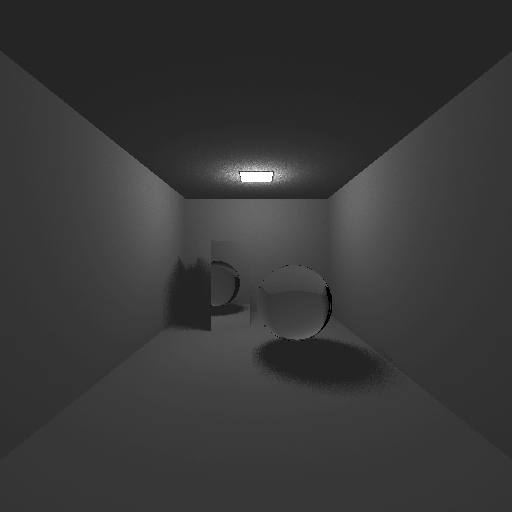
\includegraphics[width=.3\textwidth]{image/image2.png}}
    \caption{Tronclass 提供的測試影像}
    \label{fig:input}
\end{figure}

上圖(\autoref{fig:input})為 Tronclass 提供的測試影像。左側為輸入的低解析度影像(64 $\times$ 64),右側為對應的高解析度標準影像(512 $\times$ 512)。

由於我實作的三種方法皆可處理任意區塊大小 $K$,不必限定為 $N$ 的因數。因此我針對所有的整數 $K = 1 \sim 64$ 都進行測試。不過考量篇幅,這裡僅展示部分結果,即 $K = 1, 2, 4, 8, 16, 32$ 的情況。

下表(\autoref{tab:results})列出了各種方法在不同區塊大小下,與標準影像(image2.txt)相比的 MSE、PSNR、SSIM 指標。所有數值皆四捨五入至小數點後四位,其中 MSE 越小、PSNR 與 SSIM 越大代表重建結果越佳。

圖表 \autoref{fig:plot-mse}、\autoref{fig:plot-psnr}、\autoref{fig:plot-ssim} 則分別繪製三種方法在不同區塊大小 $K$ 下的 MSE、PSNR 與 SSIM 指標變化趨勢。圖組 \autoref{fig:block}、\autoref{fig:overlap}、\autoref{fig:sliding} 則分別展示三種方法在不同區塊大小下的輸出影像,以供視覺比較。

\begin{table}[h]
    \centering
    \begin{tabular}{cccc}
        \hline
        $K$ & 樣本取樣 (Block)               & 重疊取樣 (Overlap)             & 滑動視窗 (Sliding)               \\
        \hline
        1   & (0.0009, 30.27 dB, 0.9256) & (0.0004, 34.43 db, 0.9574) & (0.0009, 30.27 db, 0.9256)   \\
        \hline
        2   & (0.0007, 31.40 dB, 0.9193) & (0.0004, 34.32 db, 0.9545) & (0.0014, 28.39 db, 0.8717)   \\
        \hline
        3   & (0.0013, 28.97 dB, 0.8898) & (0.0004, 33.56 dB, 0.9473) & (0.0004, 34.43 dB, 0.957365) \\
        \hline
        4   & (0.0019, 27.23 dB, 0.8503) & (0.0005, 32.71 db, 0.9343) & (0.0004, 33.50 db, 0.9462)   \\
        \hline
        8   & (0.0113, 19.46 dB, 0.6734) & (0.0028, 25.57 db, 0.8336) & (0.0007, 31.51 db, 0.9340)   \\
        \hline
        16  & (0.0716, 11.45 dB, 0.4367) & (0.0545, 12.64 db, 0.4821) & (0.0135, 18.70 db, 0.8157)   \\
        \hline
        32  & (0.1769,  7.52 dB, 0.2118) & (0.1734,  7.61 db, 0.2165) & (0.0957, 10.19 db, 0.5112)   \\
        \hline
    \end{tabular}
    \caption{不同方法與區塊大小下的 MSE、PSNR、SSIM 比較結果}
    \label{tab:results}
\end{table}


\subsection*{結果分析}

根據上述結果,我們可以觀察到以下幾點:
\begin{itemize}
    \item 使用區塊取樣法與重疊取樣法時,選擇 $K = 1$(即直接將影像放大,不做任何插值)反而能得到較好的結果,
          但隨著 $K$ 的增加,影像品質顯著下降,容易在區塊邊緣產生 Runge 現象,導致不連續與失真。
          這是因為拉格朗日插值法較密集的取樣點會導致過擬合現象,使得插值多項式在區塊邊界處震盪劇烈。
    \item 在 $K$ 相同時,重疊取樣法普遍優於區塊取樣法,顯示出重疊取樣能有效減少區塊邊界的不連續現象。
    \item 滑動視窗法在大多數情況下表現優異,尤其在 $K$ 較大時,能夠維持較高的 PSNR 與 SSIM 指標。
          這是因為滑動視窗法能夠更平滑地處理每個像素點,減少區塊效應的影響。
    \item 使用滑動視窗法時,$K = 3$ 的效果最佳,甚至優於 $K = 1$ 與 $K = 4$ 的結果,
          這可能是因為 $K = 3$ 能夠在插值過程中提供足夠的鄰近資訊,同時避免過度擬合。
    \item 使用滑動視窗法時,$K = 2$ 時影像變得較銳利,表現不如 $K = 1$ 與 $K = 3$,
          這可能是因為 $K = 2$ 無法提供足夠的鄰近資訊,導致插值結果不夠平滑。
    \item 從圖表 \autoref{fig:plot-ssim} 可見,滑動視窗法在 SSIM 指標上明顯優於其他兩種方法,
          特別是在 $K = 32$ 時仍然可以保持約 0.5 的 SSIM 值,
          另外兩種方法在 $K = 16$ 之後 SSIM 值已下降至約 0.5 以下。
    \item 在視覺效果上,區塊取樣法與重疊取樣法在 $K \geq 8$ 時,區塊邊緣的失真與不連續現象非常明顯,
          而滑動視窗法則在 $K \geq 16$ 時,影像邊緣開始出現模糊與失真,但中央區域仍然保持較好的細節,並沒有明顯被破壞成多個區塊。
    \item 因此建議 $K$ 值應該要選擇 $3$ 或 $4$,以取得較佳的平衡點。
    \item 從圖表 \autoref{fig:compare-clamp-psnr} 與 \autoref{fig:compare-clamp-ssim} 可見,
          每次插值時進行 clamp,可能可以避免在過程中因為震盪而產生過大的值,
          但是對最終結果的 SSIM 指標沒有明顯的變化(平均差異約為 $6 \times 10^-4$),
          而對於 PSNR 值標則在 $K$ 較大時才有輕微提升(平均差異約為 $0.31$ dB),但實務上並不會選擇如此大的 $K$。
          這表明在影像重建的過程中,單純的變更 clamp 操作時機並不足以改變影像品質。
          %   然而對組數據使用成對樣本 t 檢定,得 t 統計量約 $10.6238$,p 值約為 $1.1199 \times 10^{-15}$,遠小於顯著水準 $0.05$,
          %   表示兩種方法的輸出結果在統計上仍能檢測出差異,不過
\end{itemize}

\subsection*{其他想法:正規化}

除了 clamp 操作外,我也思考過是否可以使用正規化(normalization)方法來處理插值過程中可能出現的過大或過小值。
其中一種想法是在線性正規化(linear normalization),
若果插值結果超出 $[0, 1]$ 範圍,則將整張圖片的像素值線性映射到 $[0, 1]$ 範圍內,
即對於每個像素值 $I_{ij}$,進行以下轉換:

\begin{equation}
    I_{ij}' = \frac{I_{ij} - I_{min}}{I_{max} - I_{min}}
\end{equation}

其中 $I_{min}$ 與 $I_{max}$ 分別為整張圖片的最小與最大像素值。
不過經過測試後發現,使用線性正規化反而會導致變得更糟糕,因為這會改變整張圖片的對比度與亮度分佈,例如讓影像偏白、偏暗等。
甚至在 $K = 16$ 時,因為 Runge 現象導致極端值過大,整個影像幾乎全黑。
因此我非常不建議直接使用此方法。

\begin{figure}[h]
    \centering
    \subcaptionbox{$K = 2$}{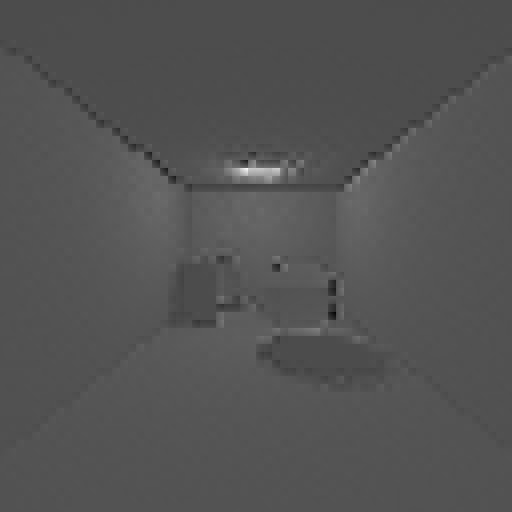
\includegraphics[width=.3\textwidth]{image/normal_K2.png}}
    \hspace{0.25cm}
    \subcaptionbox{$K = 4$}{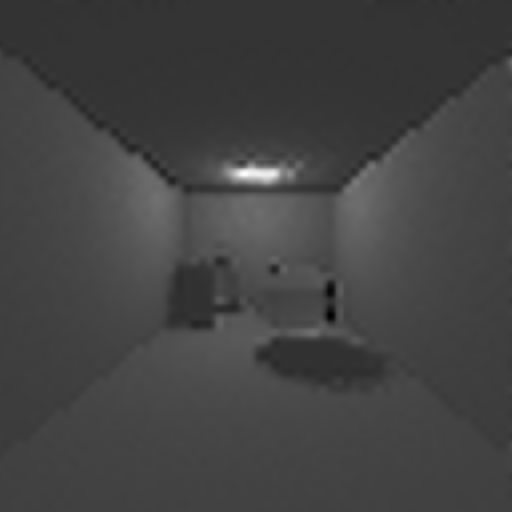
\includegraphics[width=.3\textwidth]{image/normal_K4.png}}

    \subcaptionbox{$K = 8$}{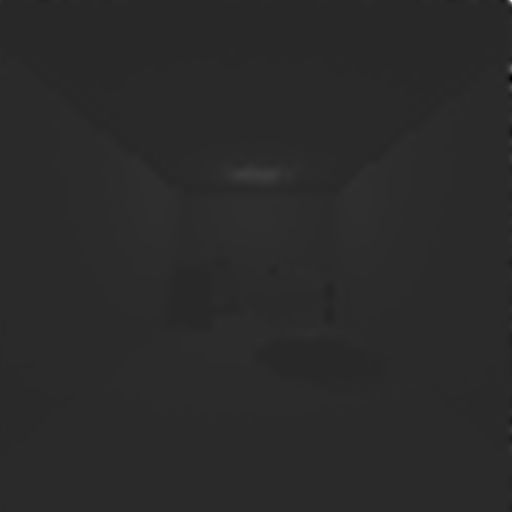
\includegraphics[width=.3\textwidth]{image/normal_K8.png}}
    \hspace{0.25cm}
    \subcaptionbox{$K = 16$}{
\includegraphics[width=.3\textwidth]{image/normal_K16.png}}
    \caption{使用線性正規化的結果}
    \label{fig:normal}
\end{figure}

此外,我也考慮了一種基於 Z-score 的非線性正規化方法。具體做法是選定某個平均值 $\mu$(如 $0.5$)與標準差 $\sigma \neq 0$,
將每個像素值 $I_{ij}$ 轉換為:

\begin{equation}
    I_{ij}' = \frac{I_{ij} - \mu}{\sigma}
\end{equation}

再透過線性正規化將結果映射到 $[0, 1]$ 範圍內。

此方法的優點在於,若插值法輸出值近似服從常態分佈,
約 $68.2 \%$ 數值將集中在 $\pm 1\sigma$ 範圍內,約 $95.7 \%$ 數值將集中在 $\pm 2\sigma$ 範圍內。
換言之,適當選擇 $\mu$ 與 $\sigma$ 可以使大部分數值集中於特定區間內,減少極端值對整體影像的影響。

然而,即便使用此方法可降低極端值的影響,影像的對比度與細節仍可能無法完全保留,並可能受到數值震盪的干擾。
由於時間有限,我並未針對此方法進行深入研究,此處僅提出作為未來可能的研究方向。

%%%%%%%%%%%%%%%%%%%%%%%%%%%%%%

\newpage

\section*{附錄:圖 \& 表}

\begin{figure}[h]
    \centering
    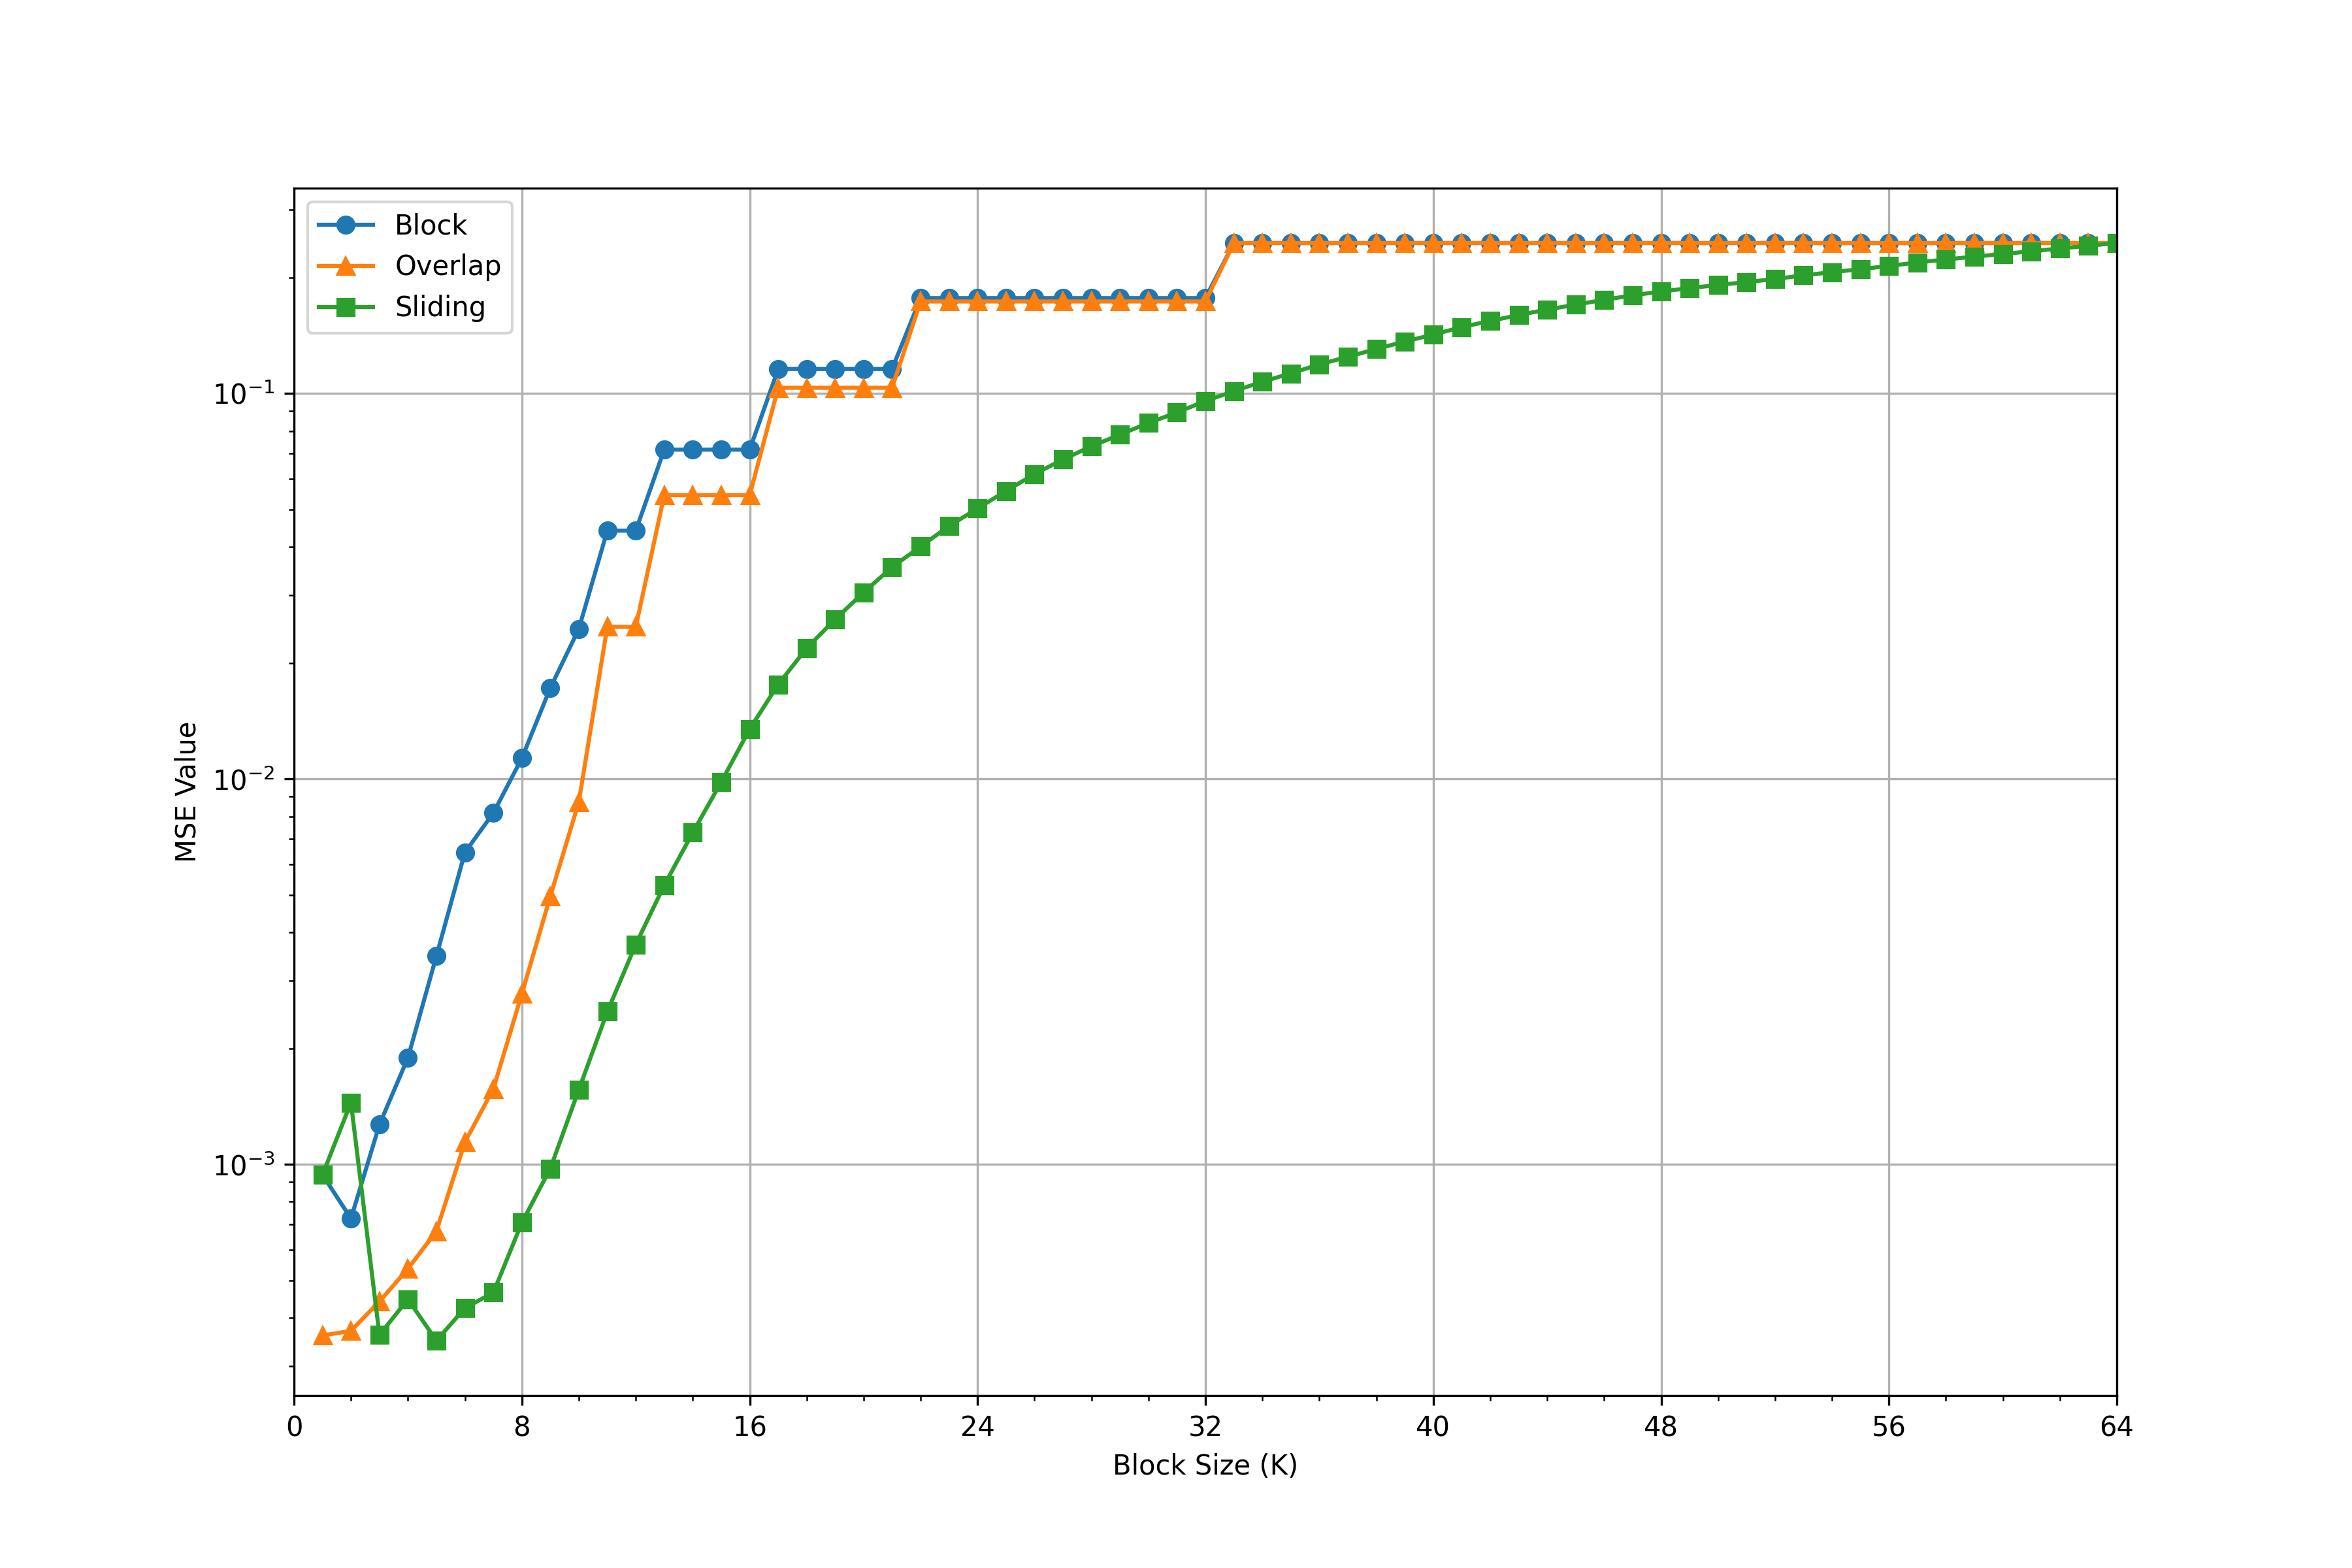
\includegraphics[width=.75\textwidth]{plots/mse.png}
    \caption{三種方法在不同區塊大小 $K$ 下的 MSE 指標比較}
    \label{fig:plot-mse}
\end{figure}

\begin{figure}[h]
    \centering
    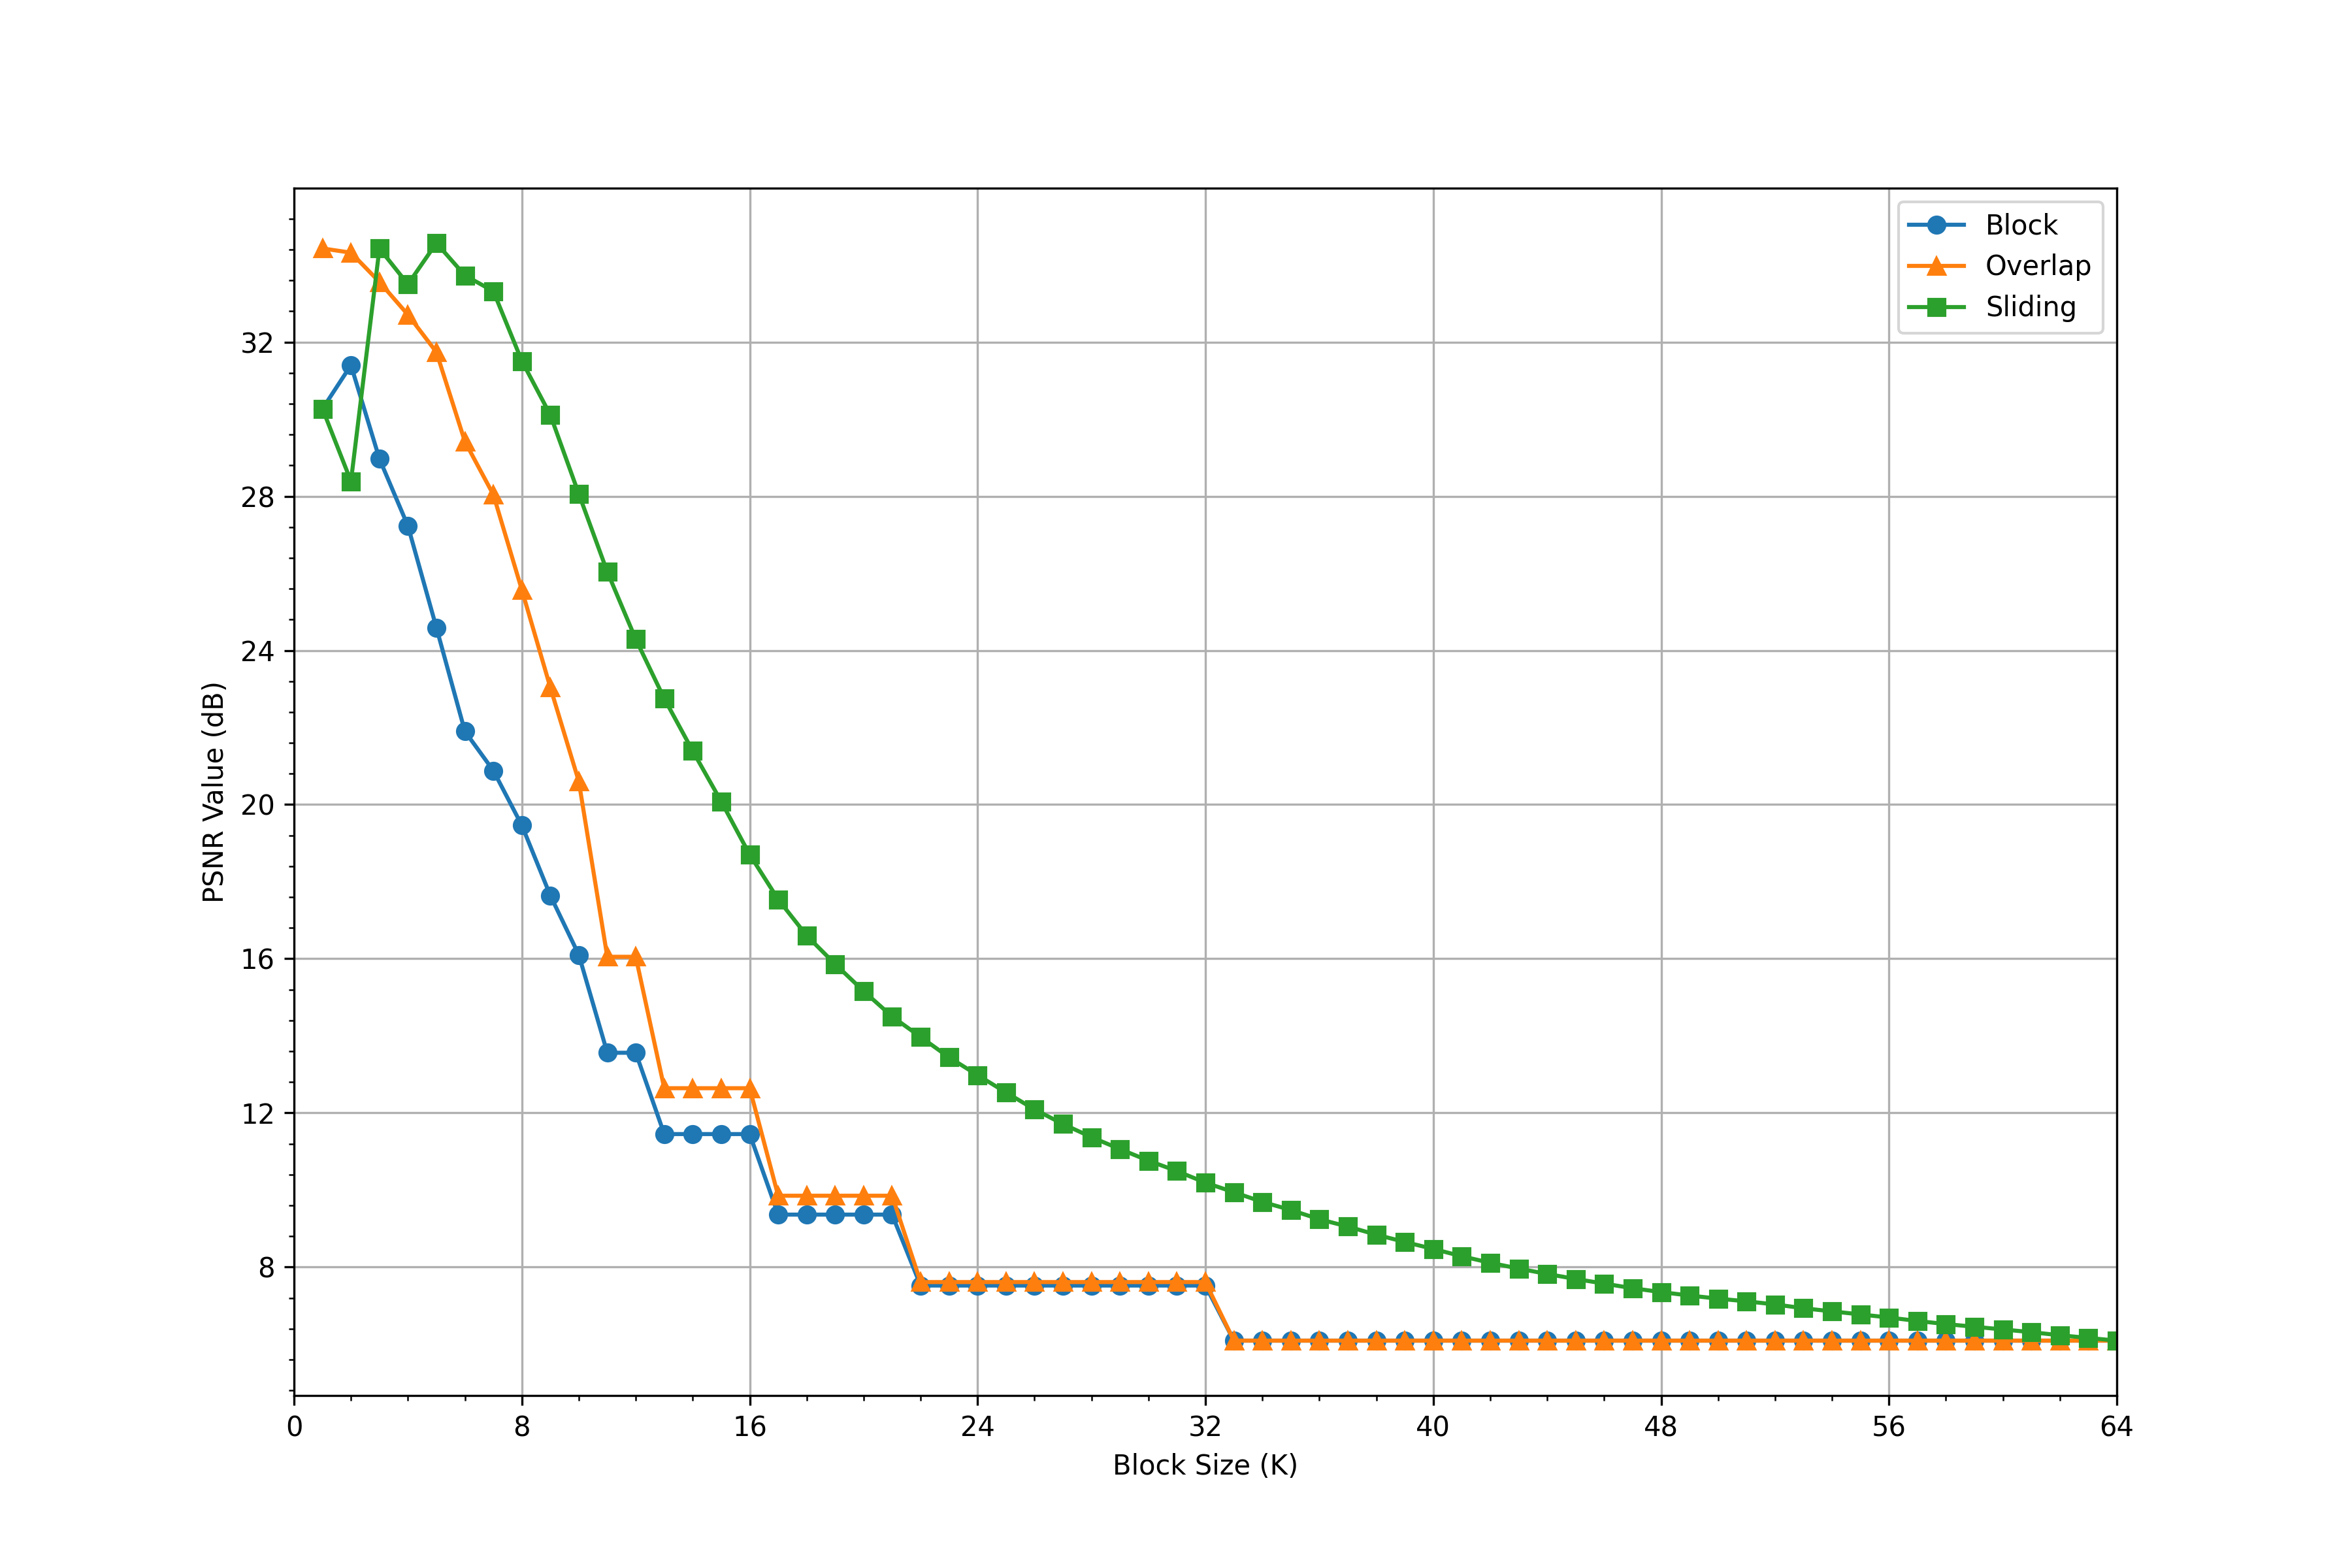
\includegraphics[width=.75\textwidth]{plots/psnr.png}
    \caption{三種方法在不同區塊大小 $K$ 下的 PSNR 指標比較}
    \label{fig:plot-psnr}
\end{figure}

\begin{figure}[h]
    \centering
    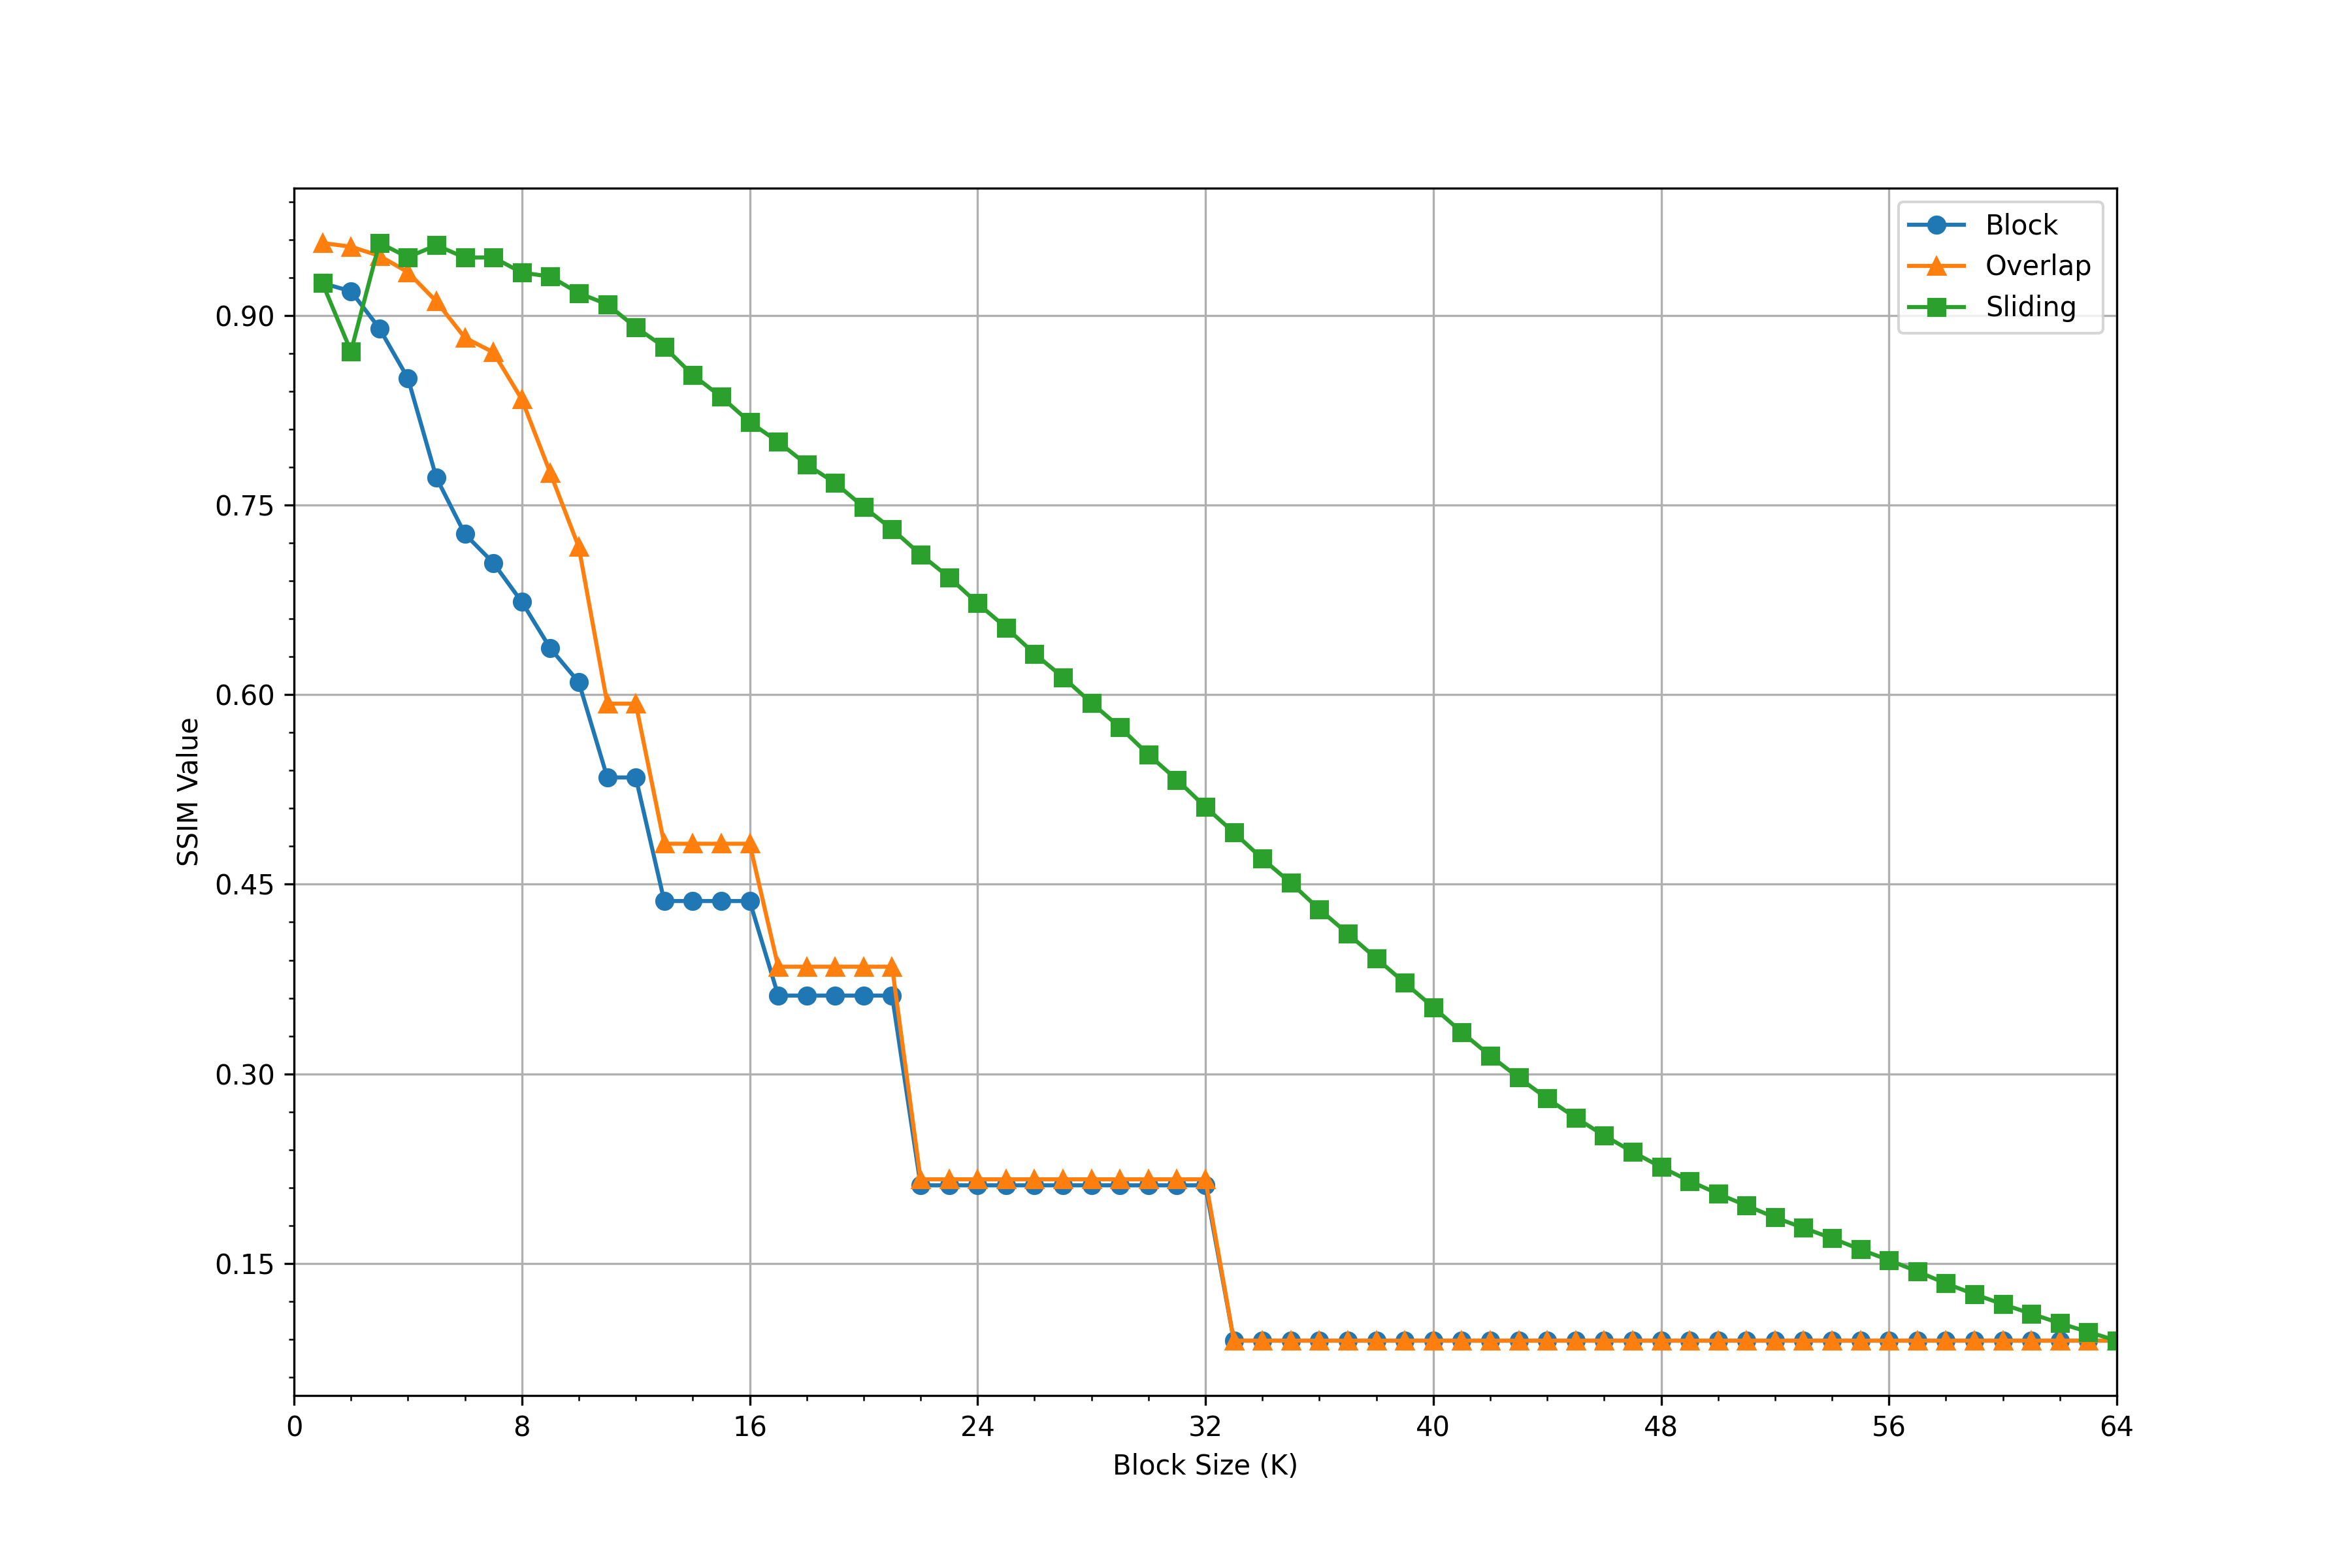
\includegraphics[width=.75\textwidth]{plots/ssim.png}
    \caption{三種方法在不同區塊大小 $K$ 下的 SSIM 指標比較}
    \label{fig:plot-ssim}
\end{figure}

\begin{figure}[h]
    \centering
    \includegraphics[width=.75\textwidth]{plots/clamp-psnr.png}
    \caption{不同 clamp 時機對 PSNR 指標的影響比較(以滑動視窗法為例)}
    \label{fig:compare-clamp-psnr}
\end{figure}

\begin{figure}[h]
    \centering
    \includegraphics[width=.75\textwidth]{plots/clamp-ssim.png}
    \caption{不同 clamp 時機對 SSIM 指標的影響比較(以滑動視窗法為例)}
    \label{fig:compare-clamp-ssim}
\end{figure}

\begin{figure}[h]
    \centering
    \subcaptionbox{$K = 1$}{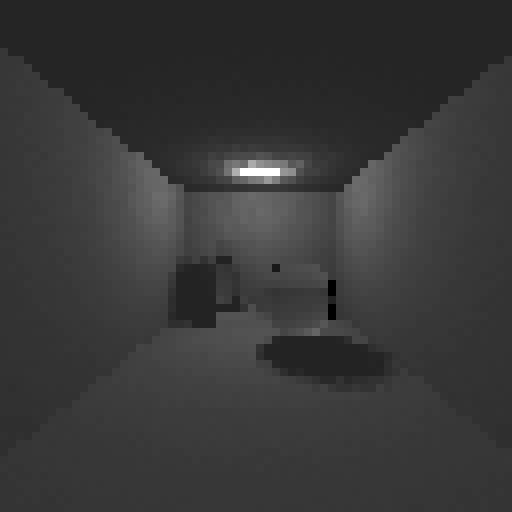
\includegraphics[width=.3\textwidth]{image/block_K1.png}}
    \hspace{0.25cm}
    \subcaptionbox{$K = 2$}{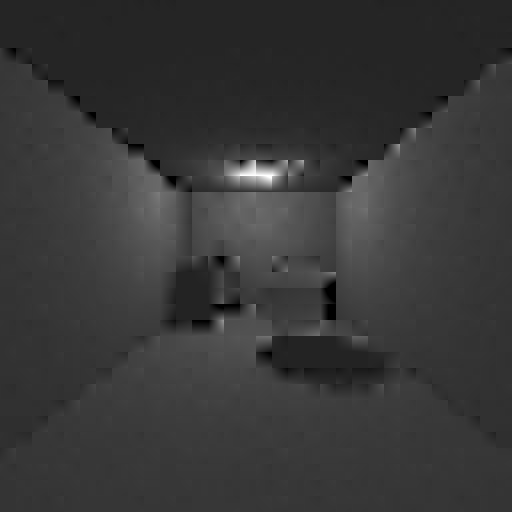
\includegraphics[width=.3\textwidth]{image/block_K2.png}}
    \hspace{0.25cm}
    \subcaptionbox{$K = 4$}{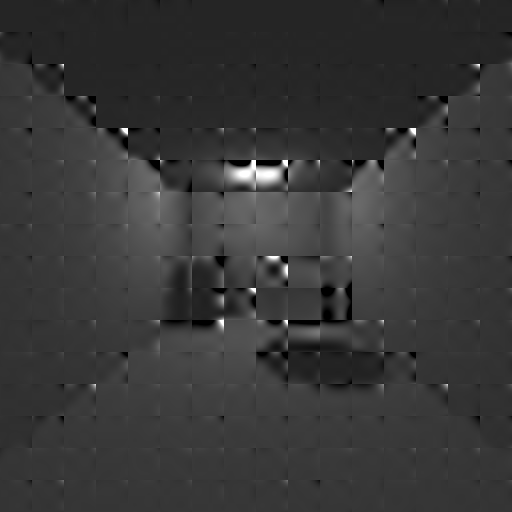
\includegraphics[width=.3\textwidth]{image/block_K4.png}}
    \hspace{0.25cm}
    \subcaptionbox{$K = 8$}{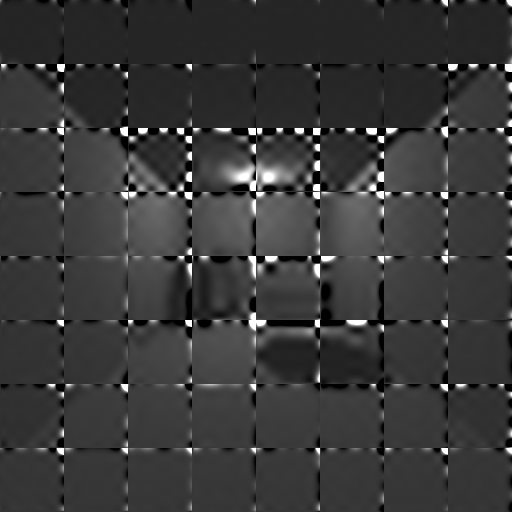
\includegraphics[width=.3\textwidth]{image/block_K8.png}}
    \hspace{0.25cm}
    \subcaptionbox{$K = 16$}{
\includegraphics[width=.3\textwidth]{image/block_K16.png}}
    \hspace{0.25cm}
    \subcaptionbox{$K = 32$}{
\includegraphics[width=.3\textwidth]{image/block_K32.png}}
    \caption{使用區塊取樣法(Block)的結果}
    \label{fig:block}
\end{figure}

\begin{figure}[h]
    \centering
    \subcaptionbox{$K = 1$}{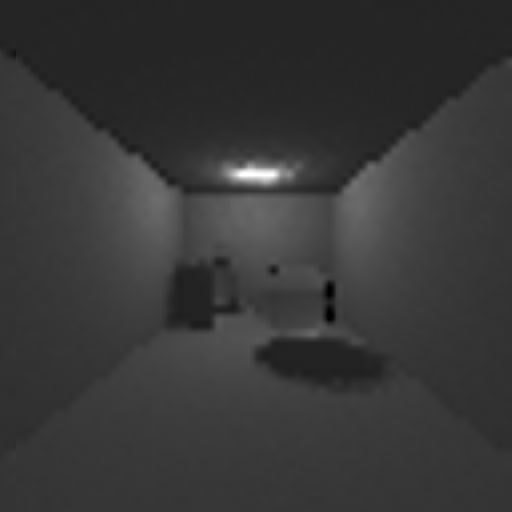
\includegraphics[width=.3\textwidth]{image/overlap_K1.png}}
    \hspace{0.25cm}
    \subcaptionbox{$K = 2$}{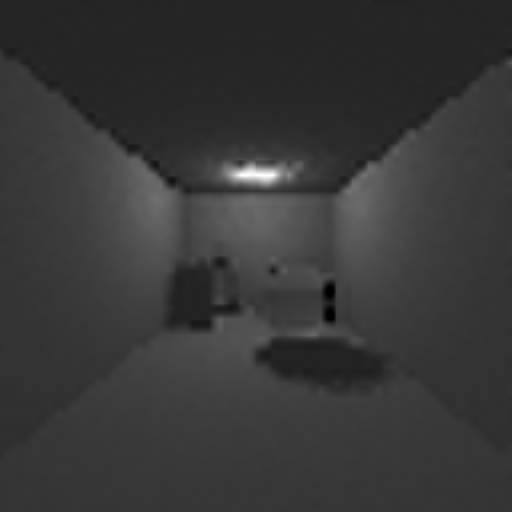
\includegraphics[width=.3\textwidth]{image/overlap_K2.png}}
    \hspace{0.25cm}
    \subcaptionbox{$K = 4$}{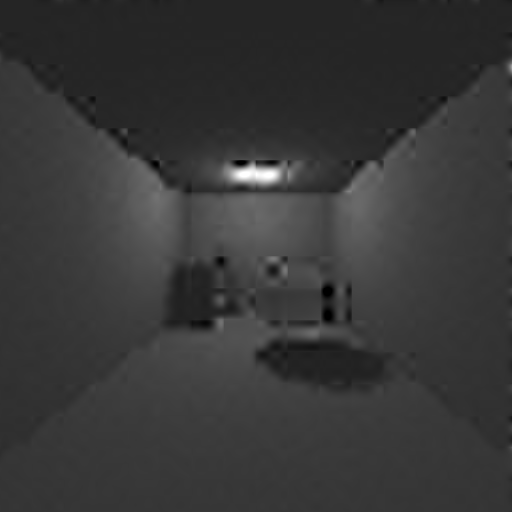
\includegraphics[width=.3\textwidth]{image/overlap_K4.png}}
    \hspace{0.25cm}
    \subcaptionbox{$K = 8$}{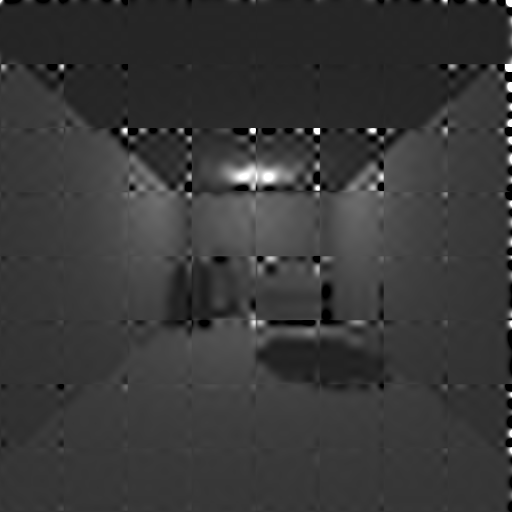
\includegraphics[width=.3\textwidth]{image/overlap_K8.png}}
    \hspace{0.25cm}
    \subcaptionbox{$K = 16$}{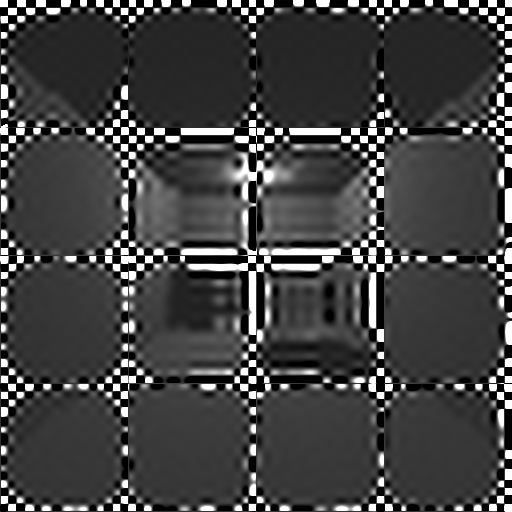
\includegraphics[width=.3\textwidth]{image/overlap_K16.png}}
    \hspace{0.25cm}
    \subcaptionbox{$K = 32$}{
\includegraphics[width=.3\textwidth]{image/overlap_K32.png}}
    \caption{使用重疊取樣法(Overlap)的結果}
    \label{fig:overlap}
\end{figure}

\begin{figure}[h]
    \centering
    \subcaptionbox{$K = 1$}{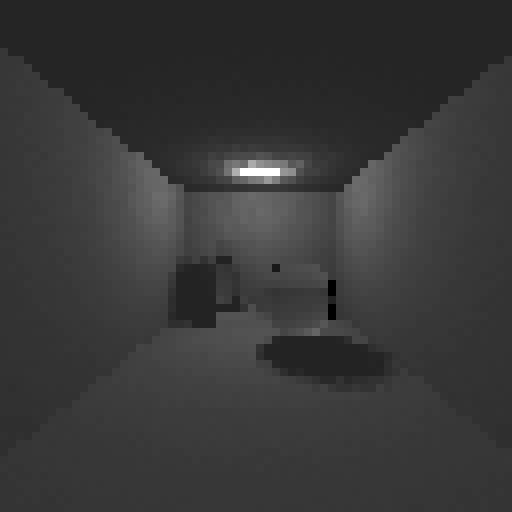
\includegraphics[width=.3\textwidth]{image/sliding_K1.png}}
    \hspace{0.25cm}
    \subcaptionbox{$K = 2$}{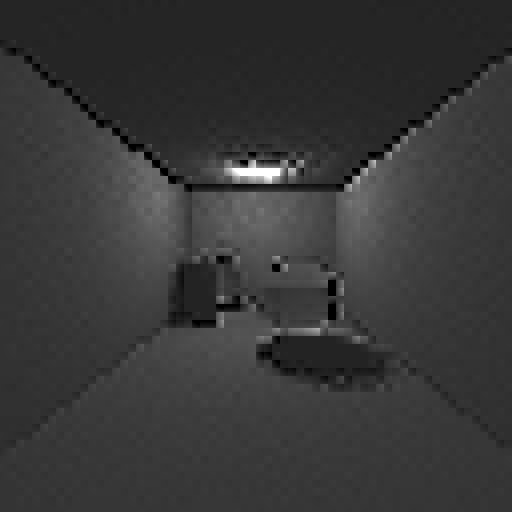
\includegraphics[width=.3\textwidth]{image/sliding_K2.png}}
    \hspace{0.25cm}
    \subcaptionbox{$K = 4$}{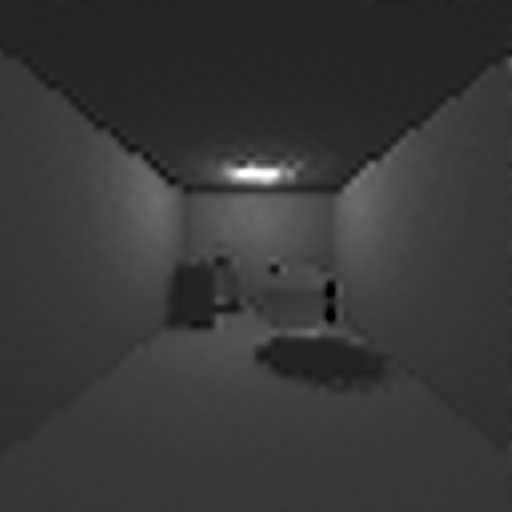
\includegraphics[width=.3\textwidth]{image/sliding_K4.png}}
    \hspace{0.25cm}
    \subcaptionbox{$K = 8$}{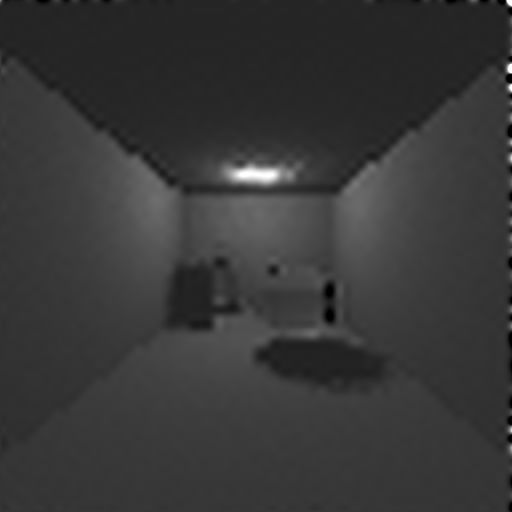
\includegraphics[width=.3\textwidth]{image/sliding_K8.png}}
    \hspace{0.25cm}
    \subcaptionbox{$K = 16$}{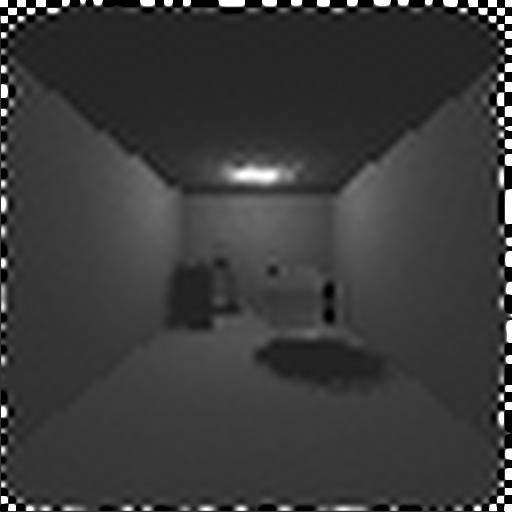
\includegraphics[width=.3\textwidth]{image/sliding_K16.png}}
    \hspace{0.25cm}
    \subcaptionbox{$K = 32$}{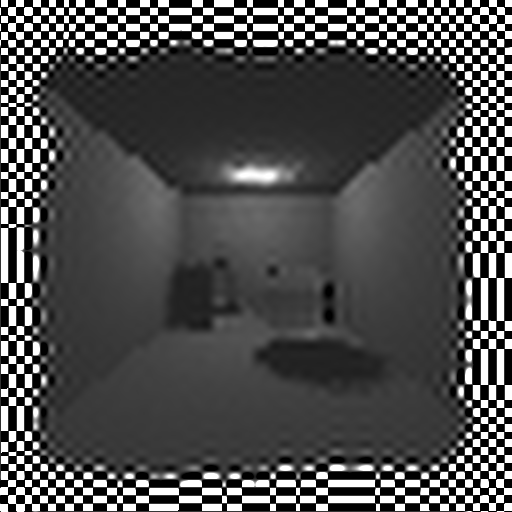
\includegraphics[width=.3\textwidth]{image/sliding_K32.png}}
    \caption{使用滑動視窗法(Sliding)的結果}
    \label{fig:sliding}
\end{figure}

\end{document}
